\section{AUTO2005 信号分析与处理 第四次作业}

提示：DFS 公式使用课件上的形式（1/N 放在正变换中），即
\[
\operatorname{DFS}[x(n)] = X(k\Omega_0) = \frac{1}{N}\sum_{n=<N>} x(n)e^{-jk\Omega_0 n}
\]

\begin{enumerate}

%======================================================================
% 第1题
%======================================================================
\item 根据题意，求解以下问题（20 分，每小题 10 分）：
\begin{enumerate}
    \item 考虑如题图 4-1 所示的周期序列 $x_p(n)$，周期 $N=4$，求该序列的 DFS；
    \begin{center}
    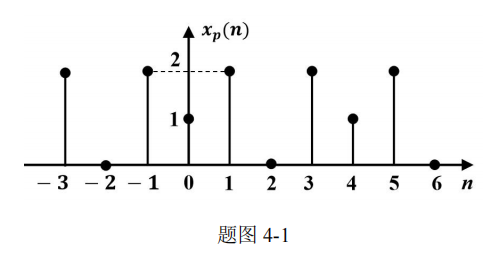
\includegraphics[width=0.4\textwidth]{4.1.png}
    \end{center}

    \textbf{解答：}

    先取一个周期 $n=0,1,2,3$ 的值：
    \[
    x_p(0)=1,\quad x_p(1)=2,\quad x_p(2)=0,\quad x_p(3)=2
    \]
    由 DFS 定义：
    \[
    X(k) = \frac{1}{4}\sum_{n=0}^{3} x_p(n)e^{-j\frac{2\pi}{4}kn}
    \]
    代入计算：
    \[
    \begin{aligned}
    X(0) &= \frac{1}{4}(1+2+0+2) = \frac{5}{4} \\
    X(1) &= \frac{1}{4}\left(1 + 2e^{-j\frac{\pi}{2}} + 0 + 2e^{-j\frac{3\pi}{2}}\right) = \frac{1}{4} \\
    X(2) &= \frac{1}{4}\left(1 + 2e^{-j\pi} + 0 + 2e^{-j3\pi}\right) = -\frac{3}{4} \\
    X(3) &= \frac{1}{4}\left(1 + 2e^{-j\frac{3\pi}{2}} + 0 + 2e^{-j\frac{\pi}{2}}\right) = \frac{1}{4}
    \end{aligned}
    \]
    即：
    \[
    X(k) = \left\{\frac{5}{4},\ \frac{1}{4},\ -\frac{3}{4},\ \frac{1}{4}\right\},\ k=0,1,2,3
    \]

    \item 考虑序号从 $n=0$ 开始的有限长序列 $x(n)=\{1,3,2,1\}$，绘出以下序列的图像，标注包括序号和幅值在内的坐标：
    \[
    x_1(n) = 0.5x((n-3))_4R_4(n),\quad x_2(n) = 2x((-n))_4R_4(n)
    \]

    \textbf{解答：}

    \begin{enumerate}
        \item 求 $x_1(n)=0.5x((n-3))_4R_4(n)$：
        先求 $x((n-3))_4$，即序列 $x(n)$ 循环右移 3 位（等价于左移 1 位）：
        \[
        x((n-3))_4R_4(n) = \{3,2,1,1\}
        \]
        乘以 0.5：
        \[
        x_1(n) = \{1.5,\ 1,\ 0.5,\ 0.5\}
        \]

        \item 求 $x_2(n)=2x((-n))_4R_4(n)$：
        先求 $x((-n))_4$，即序列 $x(n)$ 循环反褶：
        \[
        x((-n))_4R_4(n) = \{1,1,2,3\}
        \]
        乘以 2：
        \[
        x_2(n) = \{2,\ 2,\ 4,\ 6\}
        \]
    \end{enumerate}

    \vspace{0.5em}
    \textbf{序列图像：}

    \begin{center}
    \begin{tikzpicture}[>=stealth,scale=1.3]
    \draw[->] (-0.5,0) -- (4.5,0) node[right] {$n$};
    \draw[->] (0,-0.2) -- (0,2) node[above] {$x_1(n)$};
    \draw (0,0)--(0,1.5);\fill(0,1.5)circle(1.5pt);
    \draw (1,0)--(1,1);\fill(1,1)circle(1.5pt);
    \draw (2,0)--(2,0.5);\fill(2,0.5)circle(1.5pt);
    \draw (3,0)--(3,0.5);\fill(3,0.5)circle(1.5pt);
    \foreach \n in {0,1,2,3} \draw(\n,-0.05)--(\n,0.05)node[below]{$\n$};
    \node[left] at (0,1.5) {$1.5$};
    \node[left] at (0,1) {$1$};
    \node[left] at (0,0.5) {$0.5$};
    \end{tikzpicture}
    \hspace{1cm}
    \begin{tikzpicture}[>=stealth,scale=1.0]
    \draw[->] (-0.5,0) -- (4.5,0) node[right] {$n$};
    \draw[->] (0,-0.5) -- (0,7) node[above] {$x_2(n)$};
    \draw (0,0)--(0,2);\fill(0,2)circle(1.5pt);
    \draw (1,0)--(1,2);\fill(1,2)circle(1.5pt);
    \draw (2,0)--(2,4);\fill(2,4)circle(1.5pt);
    \draw (3,0)--(3,6);\fill(3,6)circle(1.5pt);
    \foreach \n in {0,1,2,3} \draw(\n,-0.1)--(\n,0.1)node[below]{$\n$};
    \node[left] at (0,2) {$2$};
    \node[left] at (0,4) {$4$};
    \node[left] at (0,6) {$6$};
    \end{tikzpicture}
    \end{center}

\end{enumerate}

\vspace{1em}

%======================================================================
% 第2题
%======================================================================
\item 考虑一个周期序列 $x(n)$，满足：
\[
x(n) =
\begin{cases}
1, & 0\le n\le 6 \\
0, & 7\le n\le 9
\end{cases}
\]
令 $g(n)=x(n)-x(n-1)$，求解以下问题：
\begin{enumerate}
    \item 证明 $g(n)$ 是周期序列，周期为 $N=10$；
    \item 求解序列 $x(n)$ 的 DFS；
    \item 求解序列 $g(n)$ 的 DFS。
\end{enumerate}

\textbf{解答：}

\begin{enumerate}
    \item 证明 $g(n)$ 周期为 $N=10$：
    因为 $x(n+10)=x(n)$，故
    \[
    g(n+10)=x(n+10)-x(n+9)=x(n)-x(n-1)=g(n)
    \]
    且 $N=10$ 是最小正周期，因此 $g(n)$ 周期为 10。

    \item 求 $x(n)$ 的 DFS：
    \[
    X(k) = \frac{1}{10}\sum_{n=0}^{9}x(n)e^{-j\frac{2\pi}{10}kn} = \frac{1}{10}\sum_{n=0}^{6}e^{-j\frac{2\pi}{10}kn}
    \]
    这是等比数列求和：
    \[
    X(k) = \frac{1}{10}\cdot \frac{1-e^{-j\frac{14\pi k}{10}}}{1-e^{-j\frac{2\pi k}{10}}} = \frac{1}{10}\cdot e^{-j\frac{6\pi k}{10}}\cdot \frac{\sin\left(\frac{7\pi k}{10}\right)}{\sin\left(\frac{\pi k}{10}\right)},\ k\neq 0
    \]
    当 $k=0$ 时：
    \[
    X(0) = \frac{7}{10}
    \]

    \item 求 $g(n)$ 的 DFS：
    由 DFS 的时移性质，$g(n)=x(n)-x(n-1)$，则
    \[
    G(k) = X(k) - e^{-j\frac{2\pi k}{10}}X(k) = X(k)\left(1-e^{-j\frac{2\pi k}{10}}\right)
    \]
    代入 $X(k)$ 即可得到 $G(k)$。
\end{enumerate}

\vspace{1em}

%======================================================================
% 第3题
%======================================================================
\item 考虑如题图 4-3 所示的 $N=4$ 有限长序列 $x(n)$，求解以下卷积和，必须写出求解过程：
\begin{center}
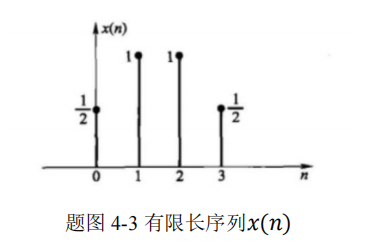
\includegraphics[width=0.4\textwidth]{4.3.png}
\end{center}
序列为：
\[
x(n) = \left\{\frac{1}{2},\ 1,\ 1,\ \frac{1}{2}\right\},\ n=0,1,2,3
\]

\begin{enumerate}
    \item $x(n)$ 与 $x(n)$ 的线性卷积；
    \item $x(n)$ 与 $x(n)$ 的 4 点圆卷积；
    \item $x(n)$ 与 $x(n)$ 的 11 点圆卷积；
    \item 欲使 $x(n)$ 与 $x(n)$ 的圆卷积和线性卷积相同，求长度 $L$ 的最小值。
\end{enumerate}

\textbf{解答：}

\begin{enumerate}
    \item 线性卷积：长度为 $4+4-1=7$。
    \[
    \begin{aligned}
    y_l(0) &= x(0)x(0) = 0.25 \\
    y_l(1) &= x(0)x(1)+x(1)x(0) = 1 \\
    y_l(2) &= x(0)x(2)+x(1)x(1)+x(2)x(0) = 2 \\
    y_l(3) &= x(0)x(3)+x(1)x(2)+x(2)x(1)+x(3)x(0) = 3 \\
    y_l(4) &= x(1)x(3)+x(2)x(2)+x(3)x(1) = 2 \\
    y_l(5) &= x(2)x(3)+x(3)x(2) = 1 \\
    y_l(6) &= x(3)x(3) = 0.25
    \end{aligned}
    \]
    \[
    y_l(n) = \{0.25,\ 1,\ 2,\ 3,\ 2,\ 1,\ 0.25\}
    \]

    \item 4 点圆卷积：
    \[
    y_c(n) = \left(\sum_{m=0}^{3}x(m)x((n-m))_4\right)R_4(n)
    \]
    计算得：
    \[
    y_c(0)=2.5,\ y_c(1)=2,\ y_c(2)=2.5,\ y_c(3)=3
    \]

    \item 11 点圆卷积：
    因为 $L=11\ge 7$，故 11 点圆卷积与线性卷积相同：
    \[
    y_{11}(n) = \{0.25,\ 1,\ 2,\ 3,\ 2,\ 1,\ 0.25,\ 0,\ 0,\ 0,\ 0\}
    \]

    \item 圆卷积与线性卷积相同的条件是 $L\ge N_1+N_2-1=4+4-1=7$，故最小长度 $L_{\min}=7$。
\end{enumerate}

\vspace{1em}

%======================================================================
% 第4题 已完善
%======================================================================
\item 已知一有限长序列
\[
h(n) =
\begin{cases}
1, & n=0 \\
-1, & n=1
\end{cases}
\]
\begin{enumerate}
    \item $x(n)=h(n)+2h(n-2)$，用 DFT 的矩阵表示式求解 $X(k)=\operatorname{DFT}[x(n)]$；
    \item 由上一问得到的 $X(k)$，求 $x(n)=\operatorname{IDFT}[X(k)]$，验证结果的正确性；
    \item 针对序列 $x(n)$ 绘制基 2 按时间抽取 FFT 算法获得自然顺序输出的蝶形运算流程图，简要分析当序列长度增加时计算复杂度的变化。
\end{enumerate}

\textbf{解答：}

\begin{enumerate}
    \item 先写出 $x(n)$：
    \[
    x(n) = \{1,\ -1,\ 2,\ -2\},\ n=0,1,2,3
    \]
    4 点 DFT 矩阵：
    \[
    W_4 = \begin{bmatrix}
    1 & 1 & 1 & 1 \\
    1 & -j & -1 & j \\
    1 & -1 & 1 & -1 \\
    1 & j & -1 & -j
    \end{bmatrix}
    \]
    \[
    X = \frac{1}{4}W_4 x = \frac{1}{4}
    \begin{bmatrix}
    0 \\
    -3+j \\
    2 \\
    -3-j
    \end{bmatrix}
    =
    \begin{bmatrix}
    0 \\
    -\frac{3}{4}+\frac{j}{4} \\
    \frac{1}{2} \\
    -\frac{3}{4}-\frac{j}{4}
    \end{bmatrix}
    \]

    \item IDFT 验证：
    \[
    x(n) = \sum_{k=0}^{3}X(k)W_4^{-kn}
    \]
    计算可得 $x(n)=\{1,-1,2,-2\}$，与原序列一致，验证正确。

    \item 基-2 按时间抽取（DIT）FFT 蝶形运算流程图：

    序列长度 $N=4=2^2$，输入先进行 \textbf{倒位序重排}：$0,1,2,3 \to 0,2,1,3$。

    \begin{center}
    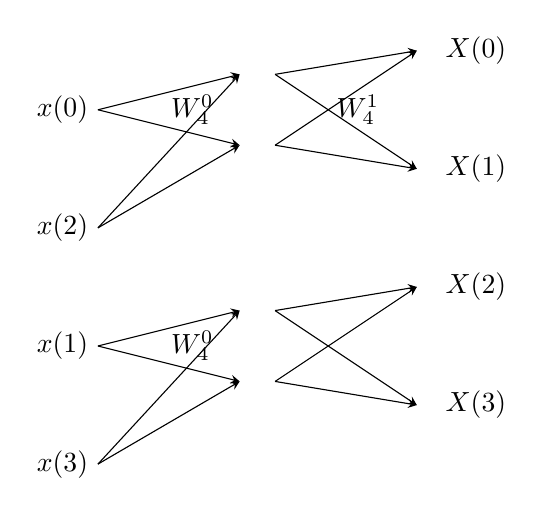
\begin{tikzpicture}[>=stealth,scale=1.5]
    % 输入节点
    \node at (0,4) {$x(0)$};
    \node at (0,3) {$x(2)$};
    \node at (0,2) {$x(1)$};
    \node at (0,1) {$x(3)$};

    % 第一级蝶形（W4^0）
    \draw[->] (0.3,4) -- (1.5,4.3);
    \draw[->] (0.3,3) -- (1.5,4.3);
    \draw[->] (0.3,4) -- (1.5,3.7);
    \draw[->] (0.3,3) -- (1.5,3.7);
    \node at (1.1,4.0) {$W_4^0$};

    \draw[->] (0.3,2) -- (1.5,2.3);
    \draw[->] (0.3,1) -- (1.5,2.3);
    \draw[->] (0.3,2) -- (1.5,1.7);
    \draw[->] (0.3,1) -- (1.5,1.7);
    \node at (1.1,2.0) {$W_4^0$};

    % 第二级蝶形（W4^0 和 W4^1）
    \draw[->] (1.8,4.3) -- (3.0,4.5);
    \draw[->] (1.8,3.7) -- (3.0,4.5);
    \draw[->] (1.8,4.3) -- (3.0,3.5);
    \draw[->] (1.8,3.7) -- (3.0,3.5);
    \node at (2.5,4.0) {$W_4^1$};

    \draw[->] (1.8,2.3) -- (3.0,2.5);
    \draw[->] (1.8,1.7) -- (3.0,2.5);
    \draw[->] (1.8,2.3) -- (3.0,1.5);
    \draw[->] (1.8,1.7) -- (3.0,1.5);

    % 输出节点
    \node at (3.5,4.5) {$X(0)$};
    \node at (3.5,3.5) {$X(1)$};
    \node at (3.5,2.5) {$X(2)$};
    \node at (3.5,1.5) {$X(3)$};
    \end{tikzpicture}
    \end{center}

    \textbf{计算复杂度分析：}
    直接 $N$ 点 DFT 的计算复杂度为 $\mathbf{O(N^2)}$；
    基‑2 FFT 算法的复杂度为 $\mathbf{O(N\log_2 N)}$。
    当序列长度 $N$ 增大时，直接 DFT 计算量呈平方级快速上升，而 FFT 仅以 $N\log_2 N$ 缓慢增长，长度越大，FFT 运算效率优势越明显。

\end{enumerate}

\vspace{1em}

%======================================================================
% 第5题 完整双方法解答
%======================================================================
\item 已知两有限长序列：
\[
x(n) = \cos\left(\frac{2\pi n}{N}\right)R_N(n),\quad h(n) = \sin\left(\frac{2\pi n}{N}\right)R_N(n)
\]
用直接卷积和 DFT 两种方法分别求以下的 $N$ 点圆周卷积：
\begin{enumerate}
    \item $y(n)=x(n)\circledast h(n)$；
    \item $y(n)=x(n)\circledast x(n)$；
    \item $y(n)=h(n)\circledast h(n)$。
\end{enumerate}

\textbf{解答：}

\textbf{方法一：DFT 方法（圆周卷积定理）}

圆周卷积定理：若 $y(n)=x(n)\circledast h(n)$，则
\[
Y(k) = N \cdot X(k)H(k)
\]
其中 $X(k)=\text{DFT}[x(n)]$，$H(k)=\text{DFT}[h(n)]$。

已知：
\[
X(k) = \frac{1}{2}\left[\delta(k-1)+\delta(k-N+1)\right]
\]
\[
H(k) = \frac{1}{2j}\left[\delta(k-1)-\delta(k-N+1)\right]
\]

\begin{enumerate}
    \item $y(n)=x(n)\circledast h(n)$
    \[
    Y(k) = N\cdot \frac{1}{2}\left[\delta(k-1)+\delta(k-N+1)\right] \cdot \frac{1}{2j}\left[\delta(k-1)-\delta(k-N+1)\right]
    \]
    \[
    Y(k) = \frac{N}{4j}\left[\delta(k-1)-\delta(k-N+1)\right]
    \]
    做 IDFT：
    \[
    y(n) = \frac{N}{2}\sin\left(\frac{2\pi n}{N}\right)R_N(n)
    \]

    \item $y(n)=x(n)\circledast x(n)$
    \[
    Y(k) = N\cdot \frac{1}{4}\left[\delta(k-1)+\delta(k-N+1)\right]^2
    \]
    \[
    Y(k) = \frac{N}{2}\delta(k) + \frac{N}{4}\left[\delta(k-1)+\delta(k-N+1)\right]
    \]
    做 IDFT：
    \[
    y(n) = \frac{N}{2}\delta(n) + \frac{N}{2}\cos\left(\frac{2\pi n}{N}\right)R_N(n)
    \]

    \item $y(n)=h(n)\circledast h(n)$
    \[
    Y(k) = N\cdot \frac{1}{-4}\left[\delta(k-1)-\delta(k-N+1)\right]^2
    \]
    \[
    Y(k) = \frac{N}{2}\delta(k) - \frac{N}{4}\left[\delta(k-1)+\delta(k-N+1)\right]
    \]
    做 IDFT：
    \[
    y(n) = \frac{N}{2}\delta(n) - \frac{N}{2}\cos\left(\frac{2\pi n}{N}\right)R_N(n)
    \]
\end{enumerate}

\textbf{方法二：直接卷积法（时域定义）}

$N$ 点圆周卷积定义：
\[
y(n) = \sum_{m=0}^{N-1}x(m)h((n-m))_N R_N(n)
\]
利用三角恒等式：
\[
\begin{aligned}
\cos A\sin B &= \frac{1}{2}[\sin(A+B)-\sin(A-B)] \\
\cos A\cos B &= \frac{1}{2}[\cos(A+B)+\cos(A-B)] \\
\sin A\sin B &= \frac{1}{2}[\cos(A-B)-\cos(A+B)]
\end{aligned}
\]
代入 $A=\frac{2\pi m}{N}, B=\frac{2\pi(n-m)}{N}$，并对 $m$ 求和，正交项求和为 0，可得：

\begin{enumerate}
    \item $y(n)=x(n)\circledast h(n)$
    \[
    y(n) = \frac{N}{2}\sin\left(\frac{2\pi n}{N}\right)R_N(n)
    \]

    \item $y(n)=x(n)\circledast x(n)$
    \[
    y(n) = \frac{N}{2}\delta(n) + \frac{N}{2}\cos\left(\frac{2\pi n}{N}\right)R_N(n)
    \]

    \item $y(n)=h(n)\circledast h(n)$
    \[
    y(n) = \frac{N}{2}\delta(n) - \frac{N}{2}\cos\left(\frac{2\pi n}{N}\right)R_N(n)
    \]
\end{enumerate}

两种方法结果一致，求解完毕。

\end{enumerate}